\documentclass[12pt,A4paper,reqno]{amsart}

%\usepackage{color,graphicx}
%\usepackage{mathrsfs,amsbsy}
\usepackage{bm}
\usepackage{booktabs}
\usepackage{ctex}
\usepackage{amssymb}
\usepackage{amsmath}
\usepackage{amsfonts}
\usepackage{array}
\usepackage{extarrows}
\usepackage{fancyhdr}
\usepackage{hhline}
\usepackage[unicode, bookmarksnumbered]{hyperref}	% 启动超链接和 PDF 文档信息所需
\usepackage{graphicx}
\usepackage{amsthm}
\usepackage{enumerate}
\usepackage[mathscr]{eucal}
\usepackage{mathrsfs}
\usepackage{mathtools}
\usepackage{verbatim}
\usepackage{wrapfig}
\usepackage{geometry} %调整页面的页边距
\usepackage{pifont}
\geometry{left=2.5cm,right=2.5cm,top=2cm,bottom=2.5cm}%具体的页边距设置
%\usepackage[notcite,notref]{showkeys}

% showkeys  make label explicit on the paper

%\makeatletter
%\@namedef{subjclassname@2010}{%
%  \textup{2010} Mathematics Subject Classification}
%\makeatother

\numberwithin{equation}{section}

\theoremstyle{plain}
\newtheorem{theorem}{Theorem}[section]
\newtheorem{lemma}[theorem]{Lemma}
\newtheorem{proposition}[theorem]{Proposition}
\newtheorem{corollary}[theorem]{Corollary}
\newtheorem{claim}[theorem]{Claim}
\newtheorem{defn}[theorem]{Definition}
\newtheorem{example}[theorem]{Example}

\theoremstyle{plain}
\newtheorem{exercise}{Exercise}[section]

\theoremstyle{plain}
\newtheorem{thmsub}{Theorem}[subsection]
\newtheorem{lemmasub}[thmsub]{Lemma}
\newtheorem{corollarysub}[thmsub]{Corollary}
\newtheorem{propositionsub}[thmsub]{Proposition}
\newtheorem{defnsub}[thmsub]{Definition}

\numberwithin{equation}{section}


\theoremstyle{remark}
\newtheorem{remark}[theorem]{Remark}
\newtheorem{remarks}{Remarks}


\newcommand*{\thick}[1]{\text{\boldmath$#1$}}
\newcommand*{\cir}[1]{\;$\ding{19#1}$\;}%临时使用
\newcommand*{\norm}[1]{\lVert#1\rVert}
\newcommand*{\pa}[2]{\partial_{#1}B_{#2}^+}
\newcommand*{\laeq}[0]{-\Delta u=f}
\newcommand*\widebar[1]{%
	\hbox{%
		\vbox{%
			\hrule height 0.5pt % The actual bar
			\kern0.35ex%         % Distance between bar and symbol
			\hbox{%
				\kern -0.1em%      % Shortening on the left side
				\ensuremath{#1}%
				\kern 0em%      % Shortening on the right side
			}%
		}%
	}%
}
%\renewcommand\thefootnote{\fnsymbol{footnote}}
%dont use number as footnote symbol, use this command to change

\DeclareMathOperator{\supp}{supp}
\DeclareMathOperator{\dist}{dist}
\DeclareMathOperator{\vol}{vol}
\DeclareMathOperator{\diag}{diag}
\DeclareMathOperator{\tr}{tr}


\begin{document}

\title[]{\LARGE S\MakeLowercase {chauder}边界估计}


\author[]{\large 周潇翔}
\address{School of Mathematical Sciences\\
University of Science and Technology of China\\
Hefei, 230026\\ P.R. China\\}
\email{xx352229@mail.ustc.edu.cn}
\maketitle




\begin{abstract}
本文的目的是较为细致地证明\cite[定理3.1]{周蜀林2019Schauder}.在此,我们追随\cite{周蜀林2019Schauder}的步伐,推导出一系列的先验估计,在此基础上证明边界估计.
\end{abstract}




%%%%%%%%%%%%%%%%%%%%%%%%%%%%%%%%%%%%%%%%%%%%%%%%%%%%%%%%%%%%%%%%%%%%%%%%%%%%%%%%%%%%%%%%%%%%%
\section{问题的提出}
我们要证明以下定理:
\begin{theorem}
	设$0< \alpha <1$.设$f \in C^{\alpha}(\widebar{B}_{1}^{+})$和$u \in C^{2}(\widebar{B}_{1}^{+})$满足
	$$\begin{cases}
	\Delta u=f & \text{ in }B_{1}^{+}\\
	\phantom{12}u=0 &\text{ on }\partial B_{1}^{+} 
	\end{cases}$$
	则$u \in C^{2,\alpha}(\widebar{B}_{1}^{+})$,且存在$C_0 >0$,使得
	\begin{align}
		[D^{2} u]_{C^{\alpha}(B_{1/2}^{+})} \leqslant C_{0}(\|f\|_{C^{\alpha}(\overline{B}_{1}^{+})}+\|u\|_{C(\overline{B}_{1}^{+})})\label{main}  \\
	\norm{u}_{C^{2,\alpha}(B_{1/2}^{+})} \leqslant C_{0}(\|f\|_{C^{\alpha}(\overline{B}_{1}^{+})}+\|u\|_{C(\overline{B}_{1}^{+})})\label{main2}
	\end{align}
	
\end{theorem}
\begin{remark}
	当(\ref{main})成立时,我们有
	\begin{equation}
		\begin{aligned}
			\norm{u}_{C^{2,\alpha}(B_{1/2}^{+})}&=	[D^{2} u]_{C^{\alpha}(B_{1/2}^{+})}+\norm{u}_{C^{2}(\overline{B}_{1/2}^{+})}\\
			&\leqslant [D^{2} u]_{C^{\alpha}(B_{1/2}^{+})}+[D^{2} u]_{C^{\alpha}(B_{1/2}^{+})}+C_1\norm{u}_{C^{2}(\overline{B}_{1/2}^{+})}&\text{\cite[引理1.1]{周蜀林2019Schauder}}\\
			&\leqslant 2C_0(\|f\|_{C^{\alpha}(\overline{B}_{1}^{+})}+\|u\|_{C(\overline{B}_{1}^{+})})+C_1\norm{u}_{C^{2}(\overline{B}_{1/2}^{+})}&\text{由(\ref{main})}\\
			&\leqslant (2C_0+C_1)(\|f\|_{C^{\alpha}(\overline{B}_{1}^{+})}+\|u\|_{C(\overline{B}_{1}^{+})})
		\end{aligned}
	\end{equation}
	故(\ref{main2})自动成立,此时$u \in C^{2,\alpha}(\widebar{B}_{1}^{+})$.故证明的关键在于(\ref{main}).
\end{remark}
	\begin{figure}[ht]
	\begin{minipage}[b]{.50\textwidth}
		为方便起见,我们引入以下符号(如图\ref{fig1}所示):
		\begin{align*}
		\pa{0}{1}&=\pa{ }{1} \cap \{x \in \mathbb{R}^n \mid x_n=0\}\\
		\pa{+}{1}&=\pa{ }{1} \cap \{x \in \mathbb{R}^n \mid x_n>0\}\\
		F&=\sup _{B_{1}^{+}} |f|
		\end{align*}
	\end{minipage}
	\begin{minipage}[b]{.33\textwidth}
		\centering
		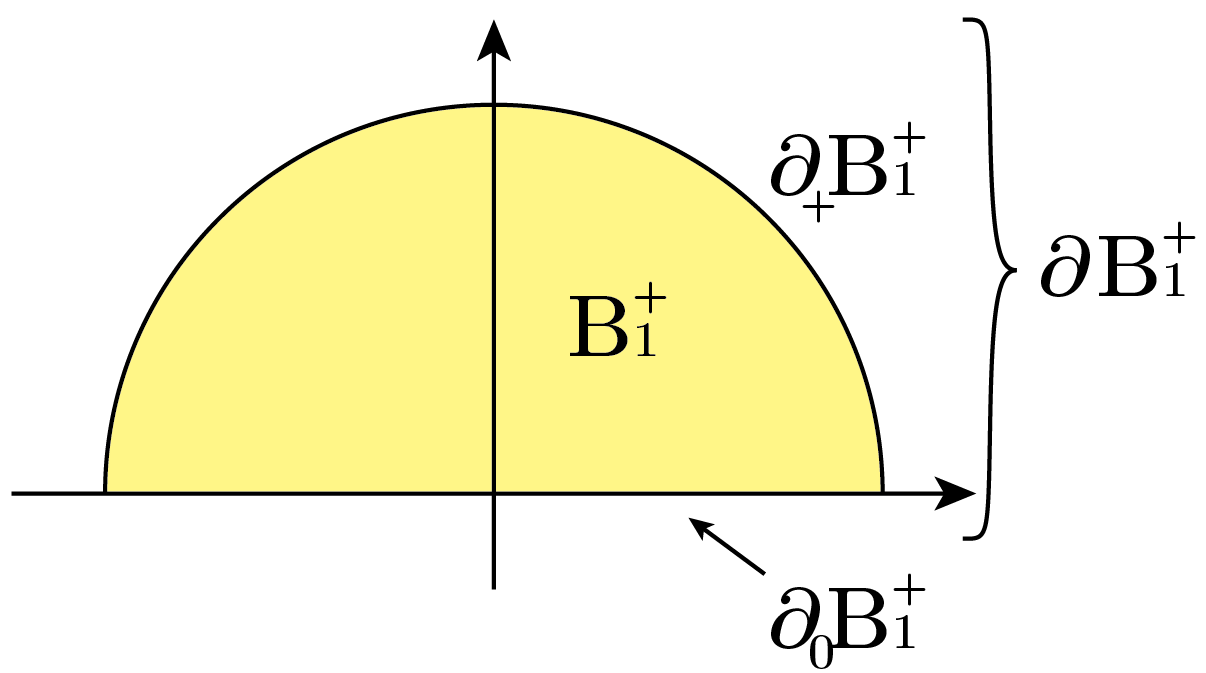
\includegraphics[width=4cm]{figures/figure1-01.png}
		\caption{}
		\label{fig1}
	\end{minipage}
\end{figure}
以下皆设$0< \alpha <1$,$C_0=C_0(n,\alpha)$为只与$n,\alpha$有关的常数,在不同的公式中可代表不同的值.

%%%%%%%%%%%%%%%%%%%%%%%%%%%%%%%%%%%%%%%%%%%%%%%%%%%%%%%%%%%%%%%%%%%%%%%%%%%%%%%%%%%%%%%%%%%%%
\section{单点估计}
\begin{lemma}
	设在半球$B_1^{+}$上有$\laeq$,则
	$$u(x) \leqslant \sup _{\partial B_{1}^{+}} u+\frac{1-|x|^{2}}{2 n} F$$
\end{lemma}
\begin{proof}
	构造函数
	$$w(x)=u(x)-\left(\sup _{\partial B_{1}^{+}} u+\frac{1-|x|^{2}}{2 n} F\right)$$
	经计算得知
	$$ -\Delta w(x) \leqslant 0, \qquad  w(x)\leqslant 0 \text{ in } \partial B_1^{+}$$
	故由极值原理\cite[定理2.22]{周蜀林2005PDE}知$w(x) \leqslant 0.$
\end{proof}
\begin{corollary}
	设在半球$B_1^{+}$上有$\laeq$,调和函数$v$满足$v=u$ on $\partial B_1^+$,则
	$$|u(x)-v(x)| \leqslant \frac{1-|x|^2}{2n}F \qquad \text{for } x \in B_1^{+}$$
\end{corollary}
下面的这个定理尝试使用一个二次调和多项式来估计函数在零点附近的情况.
\begin{theorem}\label{thm:yidian}
	存在$\varepsilon_{0}>0, \lambda \in(0,1)$,对任意满足
	$$\begin{cases}
	\laeq\\
	\sup _{B_{1}^{+}} |f|\leqslant \varepsilon_{0}\\
	\sup _{B_{1}^{+}} |u|\leqslant 1
	\end{cases}$$
	的函数$f \in C(\widebar{B}_{1}^{+})$和$u \in C^{2}(\widebar{B}_{1}^{+})$,存在一个调和多项式
	$$q(x)=\frac{1}{2}\langle A x, x\rangle+ B \cdot x+C$$
	满足:
	\begin{enumerate}
		\item $\|A\|+|B|+|C| \leqslant C_{0}$.
		\item 对所有 $x \in B_{\lambda}^{+}$, $|u(x)-q(x)| \leqslant \lambda^{2+\alpha}$.
	\end{enumerate}
\end{theorem}
\begin{proof}
	令$v$为Dirichlet问题
	$$\left\{\begin{array}{cl}{\Delta v=0,} & {x \in B_{1}} \\ {v=u,} & {x \in \partial B_{1}}\end{array}\right.$$
	的解,则:
	\begin{itemize}
		\item 由\cite[定理2.5]{周蜀林2005PDE},$$\sup _{B_{1}^{+}} |v|=\sup _{\partial B_{1}^{+}} |v|=\sup _{\partial B_{1}^{+}} |u|\leqslant \sup _{B_{1}^{+}} |u|\leqslant 1$$
		\item 由于$v|_{\partial B_1}=0$,$v$为调和函数,同\cite[Thm24, p172]{ahlfors1979complex}类似,$v$可以延拓至$B_1$(by $v(-x)=-v(x)$)且
		$$\sup _{B_{1}} |v|=\sup _{B_{1}^{+}} |v|\leqslant1$$
		\item 对任意$x \in B_{1/2}^{+},$
		$$|D^{\beta}v(x)|\leqslant C(n,|\beta|)\sup _{B_{1}} |v| \leqslant C(n,|\beta|)$$
	\end{itemize}
取$$q(x)=\frac{1}{2}\left\langle D^{2} v(0) x, x\right\rangle+ D v(0) \cdot x+v(0).$$
我们验证$q(x)$满足所需的性质:
	\begin{itemize}
	\item 由$\Delta q(x)=\Delta v(0)=0$,$q(x)$调和.
	\item $\|A\|+|B|+|C| \leqslant C_{0}$.
	\item $$v(x)-q(x)\xlongequal[t \in (0,1)]{ \exists \xi=tx}\frac{1}{3!}\left[(x \cdot D)^{3} v(\xi)\right]$$
	我们有
	\begin{align}\label{eq:estimate}
	|u(x)-q(x)|&\leqslant |u(x)-v(x)|+|v(x)-q(x)|\notag\\
	&\leqslant \frac{1-|x|^{2}}{2 n} F+C_1(n)|x|^{3} \sup _{B_1^{+}}\left|D^{3} u\right|\notag\\
	&\leqslant \frac{1}{2 n} F+C_2(n)|x|^{3}\tag{$*$}
	\intertext{其中$C_1(n),C_2(n)$是只与$n$有关的常数.}
	\intertext{取$\lambda=(2C_2(n))^{-\frac{1}{1-\alpha}},\varepsilon_{0}=n\lambda^{2+\alpha}$,则当$|x|<\lambda$时,}
	\text{ RHS of } (*)&\leqslant \frac{1}{2 n} \varepsilon_{0}+C_2(n)\lambda^{3} \leqslant \lambda^{2+\alpha}\notag
	\end{align}
	故对所有 $x \in B_{\lambda}^{+}$, $|u(x)-q(x)| \leqslant \lambda^{2+\alpha}$.
\end{itemize}
\end{proof}
\begin{theorem}\label{thm:dandian}
	设$u \in C^{2}(B_{1}^{+}) \cap C(\widebar{B}_{1}^{+}),\laeq,f$在原点处Holder连续,则存在多项式$$p(x,0)=\frac{1}{2}\langle A x, x\rangle+ B \cdot x+C$$
	满足:
	\begin{enumerate}
		\item $$\|A\|+|B|+|C| \leqslant C_{0}([f]_{\alpha, 0}+|f(0)|+\sup _{B_{1}^{+}} |u|)$$.
		\item 对所有 $x \in B_{1/2}^{+}$, $$|u(x)-p(x,0)| \leqslant C_1|x|^{2+\alpha}$$
		其中
		$$C_1\leqslant C_{0}([f]_{\alpha, 0}+|f(0)|+\sup _{B_{1}^{+}} |u|)$$
	\end{enumerate}
\end{theorem}
\begin{proof}
	不妨设
	\begin{itemize}
		\item $f(0)=0.$
		\item $|f(x)|\leqslant\varepsilon_{0}|x|^{\alpha}.$ 当$x \in B_1^{+}.$
		\item $\sup _{B_{1}^{+}} |u| \leqslant 1.$
	\end{itemize}
否则,令
$$
v(x)=u(x)-\frac{|x|^{2}}{2 n} f(0)
$$
$$
\overline{u}(x)=\varepsilon_{0} \frac{v(x)}{[f]_{\alpha, 0}+\sup _{B_{1}^{+}} |v|}
\qquad
h(x)=\varepsilon_{0} \frac{f(x)-f(0)}{[f]_{\alpha, 0}+\sup _{B_{1}^{+}} |v|}
$$
以$\overline{u},h$代替$u,f$即可.
\begin{claim}
	当$x \in B_1^{+}.$
	\item $\sup _{B_{1}^{+}} |u| \leqslant 1$时,存在一串二次调和多项式$
	p_{k}(x)=\frac{1}{2}\left\langle A_{k} x, x\right\rangle+ B_{k} \cdot x+C_{k}
	(k \in \mathbb{Z}_{\geqslant 0})$满足
	\begin{itemize}
		\item $\forall\; x \in B_{\lambda^k}^{+}$,有$$
		\left|u(x)-p_{k}(x)\right| \leqslant \lambda^{(2+\alpha) k}
		$$
		\item $$\begin{cases}
			\left\|A_{k}-A_{k-1}\right\| \leqslant C_0 \lambda^{\alpha(k-1)}\\
			\left|B_{k}-B_{k-1}\right| \leqslant C_0 \lambda^{(\alpha+1)(k-1)}\\
			\left|C_{k}-C_{k-1}\right| \leqslant C_0 \lambda^{(\alpha+2)(k-1)}
		\end{cases}$$
	\end{itemize}
\end{claim}
此时我们能够构造所需的多项式.由于${A_k},{B_k},{C_k}$是柯西列,故收敛,分别记为$A_{\infty},B_{\infty},C_{\infty}$,而
$$p(x, 0)=\frac{1}{2}\left\langle A_{\infty} x, x\right\rangle+ B_{\infty} \cdot x+C_{\infty}$$
即为所求的二次多项式.\\
固定$x \in B_{1/2}^{+}$不为零(否则显然成立),则存在$k \in \mathbb{Z}_{\geqslant 0}$使得$\lambda^{k+1}<|x| \leqslant \lambda^{k}$,此时
$$\left|p_{k}(x)-p(x, 0)\right| \leqslant C_0\left(\lambda^{\alpha k}|x|^{2}+\lambda^{(\alpha+1) k}|x|+\lambda^{(\alpha+2) k} \right)\leqslant C'_0|x|^{2+\alpha}$$
$$|u(x)-p(x, 0)| \leqslant\left|u(x)-p_{k}(x)\right|+\left|p_{k}(x)-p(x, 0)\right| \leqslant C|x|^{2+\alpha}$$
注意到之前的``不妨设"时我们所做的替换,将其替换回即可得到结论.
\end{proof}
\begin{proof}[Claim 2.5的证明]
	我们使用归纳法.\\当$k=0$时,取$p_0(x)=0$即可.当$k=1$时,取$p_1(x)$为Theorem \ref{thm:yidian} 中的二次调和多项式,则条件亦成立.\\
	下设$p_k(x)$已被构造,我们希望构造$p_{k+1}(x)$.取$w_k(x)=\frac{(u-p_{k})(\lambda^{k} x)}{\lambda^{(2+\alpha) k}}$,则$w_k(x),-\Delta w_k(x)$满足Theorem \ref{thm:yidian} 的条件,故存在一个二次调和多项式
	$q_{k}(x)=\frac{1}{2}\left\langle A_{k}^{*} x, x\right\rangle+ B_{k}^{*} \cdot x+C_{k}^{*}$
	满足
		\begin{enumerate}
		\item
		 $\|A_{k}^{*}\|+|B_{k}^{*}|+|C_{k}^{*}| \leqslant C_{0}$.
		\item 对所有 $x \in B_{\lambda}^{+}$, $|w(x)-q_{k}(x)| \leqslant \lambda^{2+\alpha}$.
	\end{enumerate}
	此时可直接验证多项式$p_{k+1}(x)=p_k(x)+\lambda^{(2+\alpha)k}q_k(\frac{x}{\lambda^k})$满足条件.
\end{proof}
%%%%%%%%%%%%%%%%%%%%%%%%%%%%%%%%%%%%%%%%%%%%%%%%%%%%%%%%%%%%%%%%%%%%%%%%%%%%%%%%%%%%%%%%%%%%%

\section{大范围的估计}
\begin{lemma}
	设$v \in \mathbb{R}^n \setminus \{0\}$,记
	$$B_1^{v}=\{x \in B_1 \vert x \cdot v >0\}$$
	存在函数$\varphi^v \in C_{0}^{\infty}\left(B_{1}^{v}\right)$使得任意$\varepsilon >0$,$P(x)$为次数小于3的多项式,有$$\varphi^v_{\varepsilon} * P=P$$
	其中$\varphi^v_{\varepsilon}(x)=\varepsilon^{-n} \varphi^v(x / \varepsilon)$.
\end{lemma}
证明可参见\cite{周蜀林2019Schauder}附录中的情形2.
\begin{theorem}\label{thm:dafan}
	设$u \in C^2(B_1^{+})$.如果存在常数$C_1>0$,$0< \alpha <1$,对任意$y \in B_{1/2}^{+}$都存在关于$x$的二次多项式$p(x,y)$满足条件
	$$
	|u(x)-p(x, y)| \leq C_{1}|x-y|^{2+\alpha}, \qquad \text{for any }x \in B_{1/4}^{+}(y) \cap B_1^{+}
	$$
	则有
	\begin{equation}
			p(x, y)=\frac{1}{2}(x-y)^{T} D^{2} u(y)(x-y)+D u(y) \cdot(x-y)+u(y)
	\end{equation}
且对于$i,j \in \{1,\ldots,n\}$,$x_1,x_2 \in B_{1/2}^{+}$,有
	\begin{equation}\label{eq:D<x}
\left|D_{i j} u\left(x_{1}\right)-D_{i j} u\left(x_{2}\right)\right| \leq C_0C_{1}\left|x_{1}-x_{2}\right|^{\alpha}
\end{equation}
\end{theorem}
\begin{proof}
	证明分3步.
	\subsection*{\underline{Step1}\vspace{-0.5cm}}
	$$\begin{cases}
	u(y)=p(y, y)\\
	D u(y)=D_{x} p(y, y)\\
	D^{2} u(y)=D_{x}^{2} p(y, y)
	\end{cases}$$
	\begin{enumerate}
		\item 显然$u(y)=p(y, y)$.
		\item \begin{equation*}
		\begin{aligned}
			D_{j} u(y)&=\lim _{h \rightarrow 0} \frac{u\left(y+h e_{j}\right)-u(y)}{h}\\
			&=\lim _{h \rightarrow 0} \frac{p\left(y+h e_{j}, y\right)-p(y, y)}{h}+\lim _{h \rightarrow 0} \frac{O\left(h^{2+\alpha}\right)}{h}\\
			&=\quad D_{x_{j}} p(y, y)
		\end{aligned}
		\end{equation*}
		故$D u(y)=D_{x} p(y, y)$.
		\item 若$\eta \in (\mathbb{R}^{n})^{+} $,记$g_{\eta}(h)=u(y+h \eta)$,则
		\begin{equation*}
		\begin{aligned}
		g_{\eta}^{\prime \prime}(0)&=\frac{1}{2} \lim _{h \rightarrow 0} \frac{g_{\eta}(h)+g_{\eta}(-h)-2 g_{\eta}(0)}{h^{2}}\\
		&=\frac{1}{2} \lim _{h \rightarrow 0} \frac{u(y+h \eta)+u(y-h \eta)-2 u(y)}{h^{2}}\\
		&=\frac{1}{2} \lim _{h \rightarrow 0} \frac{p(y+h \eta, y)+p(y-h \eta, y)-2 p(y, y)}{h^{2}}+\lim _{h \rightarrow 0} \frac{O\left(h^{2+\alpha}\right)}{h^{2}}\\
		&=D_{\eta \eta} p(x, y)
		\end{aligned}
		\end{equation*}
		而
		\begin{equation*}
		\begin{aligned}
		&g_{\eta}^{\prime \prime}(h)=\sum_{i, j=1}^{n} \eta_{i} \eta_{j} D_{i j} u(y+t \eta)\;\Rightarrow\; \begin{cases}
		g_{e_{k}}^{\prime \prime}(0)=D_{k k} u(y)\\
		g_{e_{k}+e_{l}}^{\prime \prime}(0)=D_{k k} u(y)+2 D_{k l} u(y)+D_{l l} u(y)
		\end{cases}\\
		\Rightarrow\;&D_{k l}
		 u(y)=\frac{1}{2}\left[g_{e_{k}+e_{l}}^{\prime \prime}(0)-g_{e_{k}}^{\prime \prime}(0)-g_{e_{l}}^{\prime \prime}(0)\right]=D_{kl}p(y,y)
		\end{aligned}
		\end{equation*}
		故$D^{2} u(y)=D_{x}^{2} p(y, y)$.
	\end{enumerate}
	\subsection*{\underline{Step2}}
	对$x_1,x_2 \in B_{1/2}$,当$|x_1-x_2| \leqslant \frac{1}{4}$时证明(\ref{eq:D<x}).\\
	 取$v \in \mathbb{R}^n$满足$v \cdot (x_{1}-x_{2})=0$且$v_n>0$,则对任意$z \in B_1^{+}$,有
	$$p(z,x_1)-p(z,x_2)=(p(z,x_1)-u(z))-(p(z,x_2)-u(z))$$
	取$x_0=\left(x_{1}+x_{2}\right) / 2, \varepsilon=\left|x_{1}-x_{2}\right| / 2$,两边对$\varphi_{\varepsilon}^{v}$在$B_{\varepsilon}^{+}(x_0)$做卷积,得
	$$p(z,x_1)-p(z,x_2)=[(p(\cdot,x_1)-u) *\varphi_{\varepsilon}^{v}](z) -[(p(\cdot,x_2)-u) *\varphi_{\varepsilon}^{v}](z)$$	
	两边在$x_0$处求导得
	$$D_{i j} u\left(x_{1}\right)-D_{i j} u\left(x_{2}\right)=[(p(\cdot,x_1)-u) *D_{i j}\varphi_{\varepsilon}^{v}](z) -[(p(\cdot,x_2)-u) *D_{i j}\varphi_{\varepsilon}^{v}](z)$$
	而
	\begin{equation*}
	\begin{aligned}
		\biggl|[(p(\cdot,x_1)-u) *D_{i j}\varphi_{\varepsilon}^{v}](z)\biggr|&\leqslant\varepsilon^{-n-2} \int_{\substack{|y-x|<\varepsilon \\ (y-x)\cdot v>0}}\left|u(y)-p\left(y, x_1\right)\right|\biggl| D_{i j} \varphi^{v}(\frac{x-y}{\varepsilon})\biggr| d y\\
		&\leqslant \varepsilon^{-n-2}\sup_{B_{1}}|D_{i j} \varphi^{v}| \int_{A_{x_1}}\left|u(y)-p\left(y, x_1\right)\right| d y\\
		&\leqslant \varepsilon^{-n-2}\sup_{B_{1}}|D_{i j} \varphi^{v}|C_1 \int_{A_{x_1}}\left|y-x_1\right|^{2+\alpha} d y\\
		&\leqslant C'_0C_1 \varepsilon^{\alpha}\\
		&= C_0C_1 |x_2-x_1|^{\alpha}\\
	\end{aligned}
	\end{equation*}
	同理
	$$\biggl|[(p(\cdot,x_2)-u) *D_{i j}\varphi_{\varepsilon}^{v}](z)\biggr|\leqslant C_0C_1 |x_2-x_1|^{\alpha}$$
	从而得到(\ref{eq:D<x}).
	\begin{figure}[th]
		\centering
		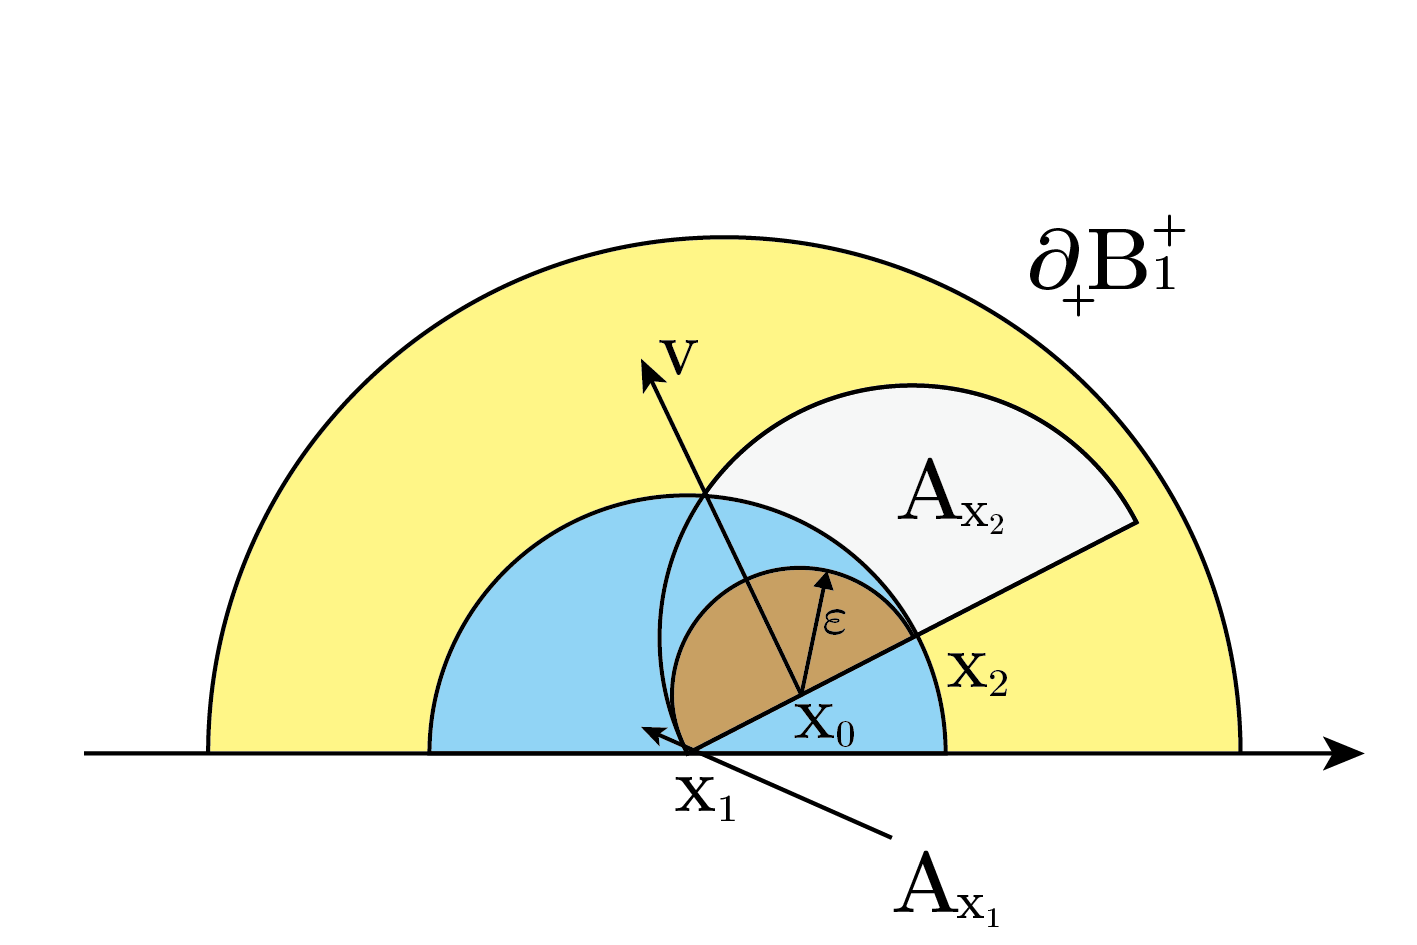
\includegraphics[width=0.6\textwidth]{figures/figure3-01.png}\\
		\caption{}
	\end{figure}
	\subsection*{\underline{Step3}}
	对一般的$x_1,x_2 \in B_{1/2}$证明(\ref{eq:D<x}).\\
	取$z_i=x_1+\frac{i}{4}(x_2-x_1)\; (i=0,1,2,3,4)$,对$(z_0,z_1),\ldots,(z_3,z_4)$分别应用Step2即可.
\end{proof}
%%%%%%%%%%%%%%%%%%%%%%%%%%%%%%%%%%%%%%%%%%%%%%%%%%%%%%%%%%%%%%%%%%%%%%%%%%%%%%%%%%%%%%%%%%%%%

\section{原命题的证明}
现在我们可以证明主定理:
\begin{theorem}
	设$0< \alpha <1$.设$f \in C^{\alpha}(\widebar{B}_{1}^{+})$和$u \in C^{2}(\widebar{B}_{1}^{+})$满足
	$$\begin{cases}
	\Delta u=f & \text{ in }B_{1}^{+}\\
	\phantom{12}u=0 &\text{ on }\partial B_{1}^{+} 
	\end{cases}$$
	则$u \in C^{2,\alpha}(\widebar{B}_{1}^{+})$,且存在$C_0 >0$,使得
	\begin{align}
	[D^{2} u]_{C^{\alpha}(B_{1/2}^{+})} \leqslant C_{0}(\|f\|_{C^{\alpha}(\overline{B}_{1}^{+})}+\|u\|_{C(\overline{B}_{1}^{+})})  \\
	\norm{u}_{C^{2,\alpha}(B_{1/2}^{+})} \leqslant C_{0}(\|f\|_{C^{\alpha}(\overline{B}_{1}^{+})}+\|u\|_{C(\overline{B}_{1}^{+})})
	\end{align}
	
\end{theorem}
		\begin{figure}[ht]
		\begin{minipage}[b]{.65\textwidth}
				证明:固定$y \in B_{1/2}^{+}$,令$$r=\operatorname{dist}\left(y, \partial_+ B_{1}\right)>1/2,$$$$v(x)=u(y+r x),\quad g(x)=r^{2} f(y+r x)\;(x \in B_1^{+}),$$则在$B_1^{+}$上,$-\Delta v=g$满足Theorem \ref{thm:dandian} 的条件,故存在二次多项式$p_0(x)$满足 
			\begin{equation}\label{equ:aa}
			|v(x)-p_0(x)| \leqslant C_1|x|^{2+\alpha}\;\text{ for any }x \in B_{1/2}^{+}
			\end{equation}
			其中
			$$C_1\leqslant C_{0}([g]_{\alpha, 0}+|g(0)|+\sup _{B_{1}^{+}} |v|)$$
			取$q(x,y)=p_0((x-y)/r)$,我们通过对(\ref{equ:aa})的变形验证$q(x,y)$满足Theorem \ref{thm:dafan} 的条件:
		\end{minipage}
		\begin{minipage}[b]{.33\textwidth}
			\centering
			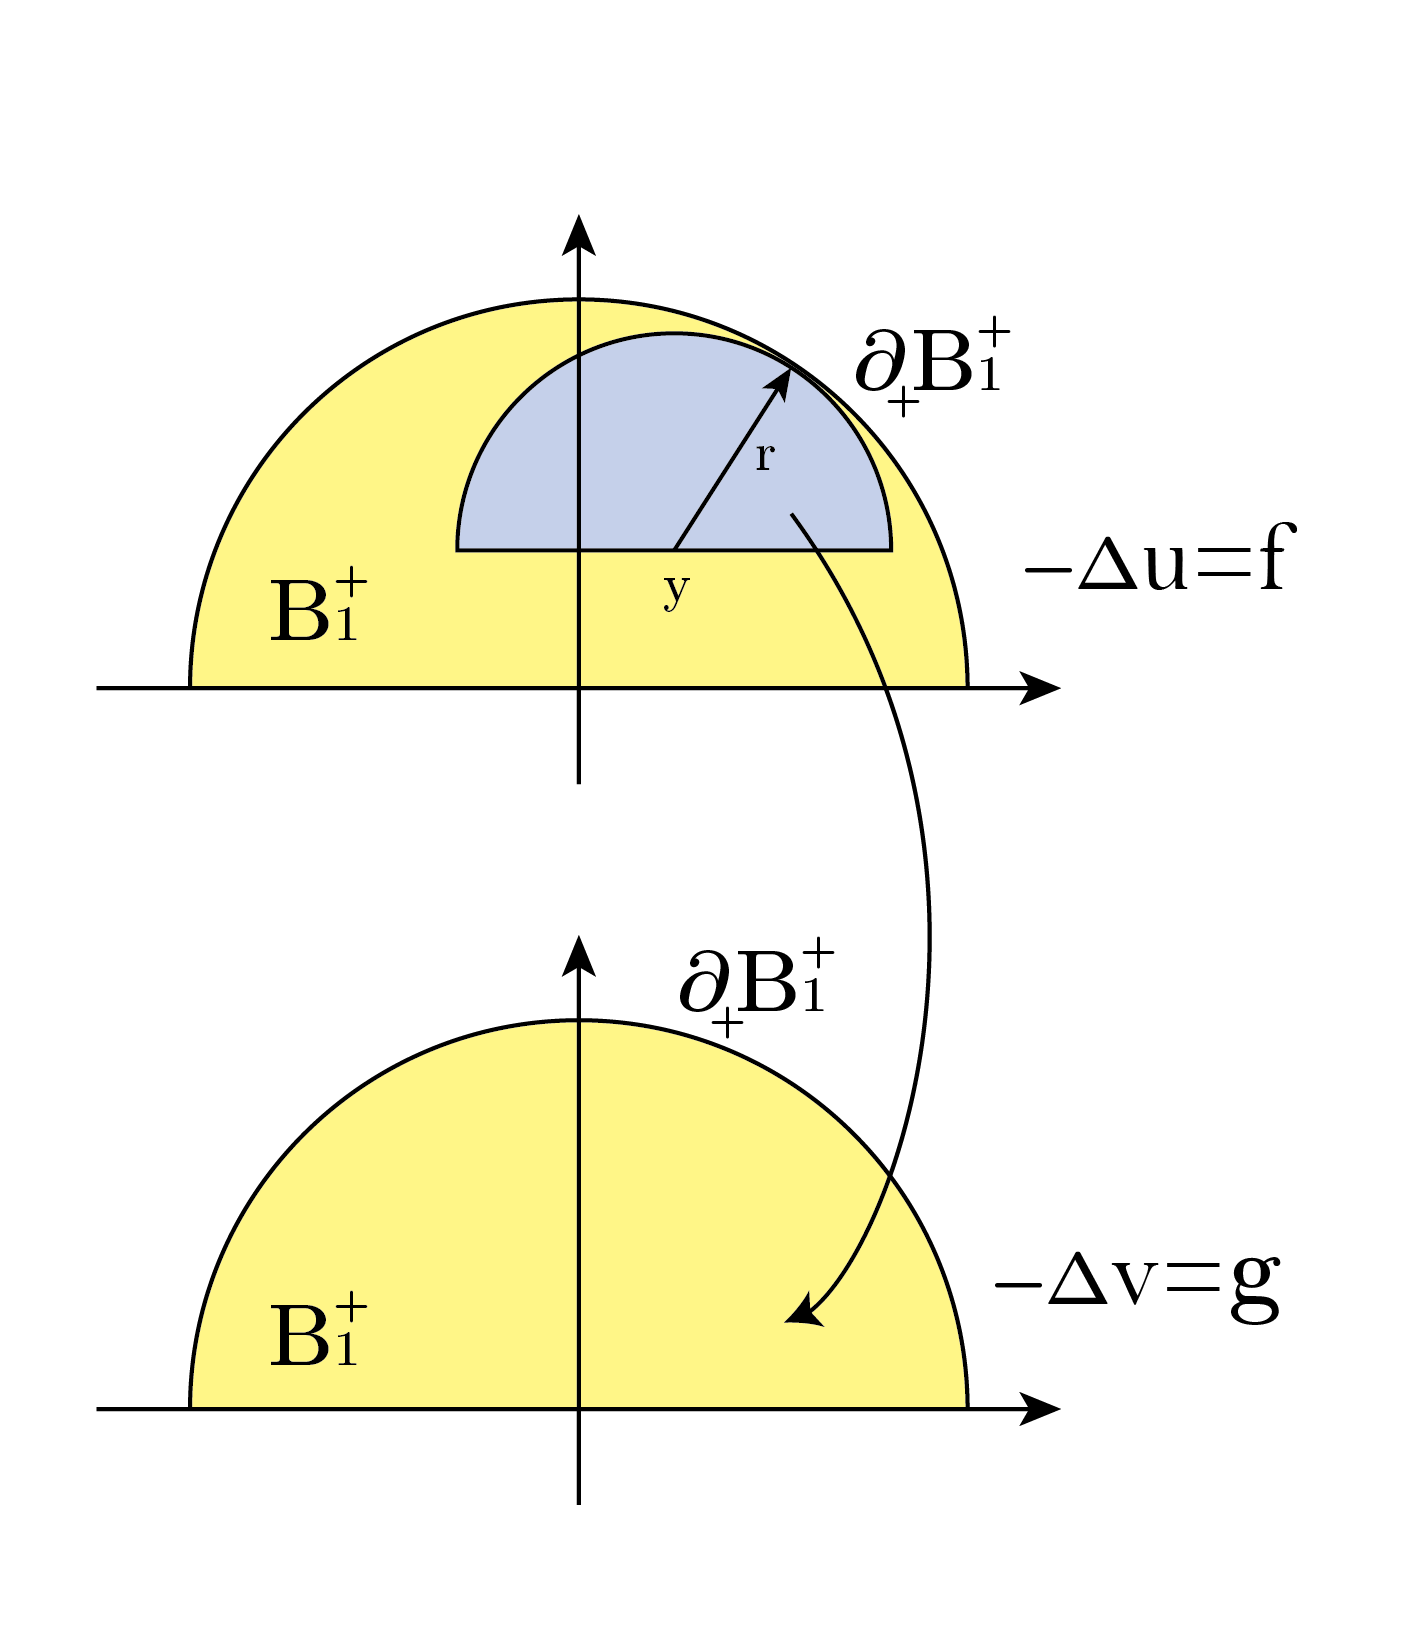
\includegraphics[width=5cm]{figures/figure2-01.png}
			\caption{}
		\end{minipage}
	\end{figure}\vspace{-1cm}
	$$|u(x)-q(x,y)|\leqslant C^{*}_1|x|^{2+\alpha}\qquad\text{ for any } z \in B_{1/4}^{+}(y) \subseteq B_{r/2}^{+}(y)$$
	其中$C_1^{*}\leqslant C_0([f]_{\alpha, 0}+\sup _{B_{1}^{+}} |v|+\sup _{B_{1}^{+}} |u|)$.\\
	故而有
	$$\left|D_{i j} u\left(x_{1}\right)-D_{i j} u\left(x_{2}\right)\right| \leq C'_0C_1^{*}\left|x_{1}-x_{2}\right|^{\alpha}$$
	原命题得证.
%%%%%%%%%%%%%%%%%%%%%%%%%%%%%%%%%%%%%%%%%%%%%%%%%%%%%%%%%%%%%%%%%%%%%%%%%%%%%%%%%%%%%%%%%%%%%
\section{致谢}
特别感谢北大的李泽兴学长,他教会了我很多如何将内估计推广到边界估计的办法.可以说这篇小论文中大部分新颖的点子都是他想出来的,没有他我就真的无法完成大作业了.
%%%%%%%%%%%%%%%%%%%%%%%%%%%%%%%%%%%%%%%%%%%%%%%%%%%%%%%%%%%%%%%%%%%%%%%%%%%%%%%%%%%%%%%%%%%%%





%%%%%%%%%%%%%%%%%%%%%%%%%%%%%%%%%%%%%%%%%%%%%%%%%%%%%%%%%%%%%%%%%%%%%%%%%%






%%%%%%%%%%%%%%%%%%%%%%%%%%%%%%%%%%%%%%%%%%%%%%%%%%%%%%%%%%%%%%%%%%%%%%%%%%%%%%%%%%%%%%%%%%%%%%%





\bibliographystyle{plain}
\bibliography{reference}
\nocite{gilbarg2015elliptic}
\nocite{陈亚浙1991}
\nocite{calderon1989local}
\end{document}




